\documentclass[t,handout]{beamer}
\usepackage[default]{sourcesanspro}
% \usepackage[default]{sourcecodepro}
% \usepackage[default]{sourceserifpro}
\usepackage[utf8]{inputenc}
\usepackage[english]{babel}
\usepackage{listings}
\lstset{ %
  basicstyle=\ttfamily\color{black}\tiny,
  breaklines=true,
  columns=fullflexible,
  frame=single,
  keepspaces=true,
  tabsize=2
}

\definecolor{darkblue}{rgb}{0,0,.5}
\hypersetup{pdftex=true, colorlinks=true, breaklinks=true, linkcolor=darkblue, menucolor=darkblue, pagecolor=darkblue, urlcolor=darkblue}

\title{Taskwarrior -- What's next?}
\subtitle{The Taskwarrior Universe}
\author[Deimeke, Dirk]{Dirk Deimeke}
\institute[Taskwarrior Academy]{Taskwarrior Academy}
\date{2016}
\titlegraphic{
\includegraphics[width=3cm,height=3cm]{tw-xxl}}
\subject{Taskwarrior}
\keywords{taskwarrior, task, management, commandline, getting things done}

\setbeamercovered{transparent}

\pgfdeclareimage[width=5mm]{tw-logo}{tw-xl}

%%%%%%%%%%%%%%%%%%%%%%%%%%%%%%%%%%%%%%%%%%%%%%%%%%%%%%%%%%%%%%%%%%%%%%%
%
% LaTeX-Template for Taskwarrior by Dominik Wagenführ
% http://www.deesaster.org/
%
% Creative Commons Attribution-ShareAlike 4.0 (CC-BY-SA 4.0)
% https://creativecommons.org/licenses/by-sa/4.0/
%
%%%%%%%%%%%%%%%%%%%%%%%%%%%%%%%%%%%%%%%%%%%%%%%%%%%%%%%%%%%%%%%%%%%%%%%

%%%%%%%%%%%%%%%%%%%%%%%%%%%
% Layout - Start
%%%%%%%%%%%%%%%%%%%%%%%%%%%

\setbeamertemplate{navigation symbols}{}

\useinnertheme{default}
\useoutertheme{infolines}
\usefonttheme{structurebold}

\newlength{\boxwidth}
\setlength{\boxwidth}{121px}
\setbeamertemplate{headline}{%
\begin{beamercolorbox}[dp=3px,ht=6px,wd=\boxwidth,center]{palette tertiary}%
\insertauthor\ (\insertinstitute)%
\end{beamercolorbox}%
\vskip-9px\hskip\boxwidth
\begin{beamercolorbox}[dp=3px,ht=6px,wd=\boxwidth,center]{palette secondary}%
\inserttitle%
\end{beamercolorbox}%
\begin{beamercolorbox}[dp=3px,ht=6px,wd=\boxwidth,right]{palette primary}%
\insertdate\hskip15px\insertframenumber\,/\,\inserttotalframenumber\hspace*{8px}
\end{beamercolorbox}%
}
\setbeamertemplate{footline}{}

%%%%%%%%%%%%%%%%%%%%%%%%%%%
% Colors - Start
%%%%%%%%%%%%%%%%%%%%%%%%%%%

\definecolor{basecolor}{gray}{0.2}
\definecolor{mittelgrau}{gray}{0.4}
\definecolor{hellgrau}{gray}{0.93}
\definecolor{gelb}{rgb}{1.0,1.0,0.75}

% infolines color
\setbeamercolor{palette primary}{fg=white,bg=mittelgrau}
\setbeamercolor{palette secondary}{fg=white,bg=basecolor}
\setbeamercolor{palette tertiary}{fg=white,bg=black}

% frame and title color
\setbeamercolor{frametitle}{fg=white,bg=basecolor}
\setbeamercolor{titlelike}{fg=white,bg=basecolor}
\setbeamerfont{frametitle}{series=\bfseries}

% TOC color
\setbeamercolor{section in toc}{fg=basecolor}

% text color
\setbeamercolor{normal text}{fg=black,bg=white}

% item color
\setbeamercolor{item}{fg=basecolor}
\setbeamercolor{itemize item}{fg=black}

% block color
\setbeamercolor{block title}{fg=black,bg=gelb}
\setbeamercolor{block body}{fg=black,bg=gelb}

% block alert color
\setbeamercolor{block title alerted}{fg=black,bg=gelb}
\setbeamercolor{block body alerted}{fg=black,bg=gelb}

% block example color
\setbeamercolor{block title example}{fg=black,bg=gelb}
\setbeamercolor{block body example}{fg=black,bg=gelb}

\setbeamertemplate{frametitle}{%
\vskip-1px%
\begin{beamercolorbox}[wd=363px,ht=20px,dp=12px]{frametitle}
\usebeamerfont{frametitle}%
\usebeamercolor{frametitle}%
\vspace*{-5px}\hspace*{10px}
\includegraphics[width=24px,height=24px]{tw-xl.png}\\
\vspace*{-20px}\hspace*{40px}\insertframetitle%
\end{beamercolorbox}
}

%%%%%%%%%%%%%%%%%%%%%%%%%%%
% Colors - Stop
%%%%%%%%%%%%%%%%%%%%%%%%%%%

%%%%%%%%%%%%%%%%%%%%%%%%%%%%%%%%%%%%%%%%%%%%%%%%%%%%%%%%%%%%%%%%%%%%%%%

\begin{document}

\begin{frame} % Titel
	\titlepage
\end{frame}

% \logo{\pgfuseimage{tw-logo}}

%\begin{frame}\frametitle{Content}
%	\tableofcontents
%\end{frame}

%%%%%%%%%%%%%%%%%%%%%%%%%%%
\section{Ressources}
%%%%%%%%%%%%%%%%%%%%%%%%%%%

\begin{frame}\frametitle{Support}
    \vfill
    \begin{itemize}
        \item \href{https://answers.tasktools.org/}{answers.tasktools.org}
        \item \href{mailto:support@taskwarrior.org}{support@taskwarrior.org}
        \item \#taskwarrior on freenode.net
        \item @taskwarrior on Twitter
        \item \href{https://groups.google.com/forum/\#!forum/taskwarrior-dev}{Developer Mailinglist}
        \item \href{https://groups.google.com/forum/\#!forum/taskwarrior-user}{User Mailinglist}
    \end{itemize}
\end{frame}

\begin{frame}\frametitle{Contribute to Taskwarrior}
    \vfill
    \href{http://taskwarrior.org/docs/contribute.html}{Want to contribute?}
    \vfill
	\begin{alertblock}{How to become an Open Source Contributor}
		We have some information for you on how to become an Open Source Contributor for the \href{http://taskwarrior.org/docs/first_time.html}{first time} (applies to the second and third contribution as well).
	\end{alertblock}
\end{frame}

\begin{frame}\frametitle{taskwarrior.org -- main page}
    \begin{center}
        \href{http://taskwarrior.org}{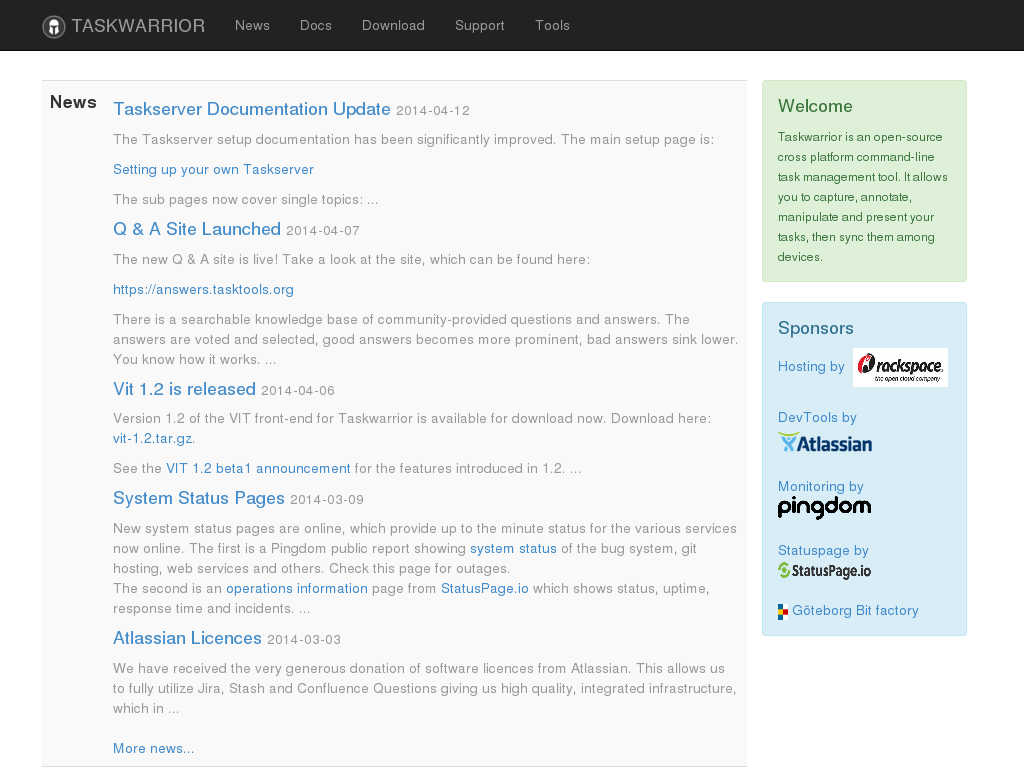
\includegraphics[width=10cm,height=7.5cm]{taskwarrior-org.png}}
    \end{center}
\end{frame}

\begin{frame}\frametitle{answers.tasktools.org -- Questions and answers}
    \begin{center}
        \href{http://answers.tasktools.org/}{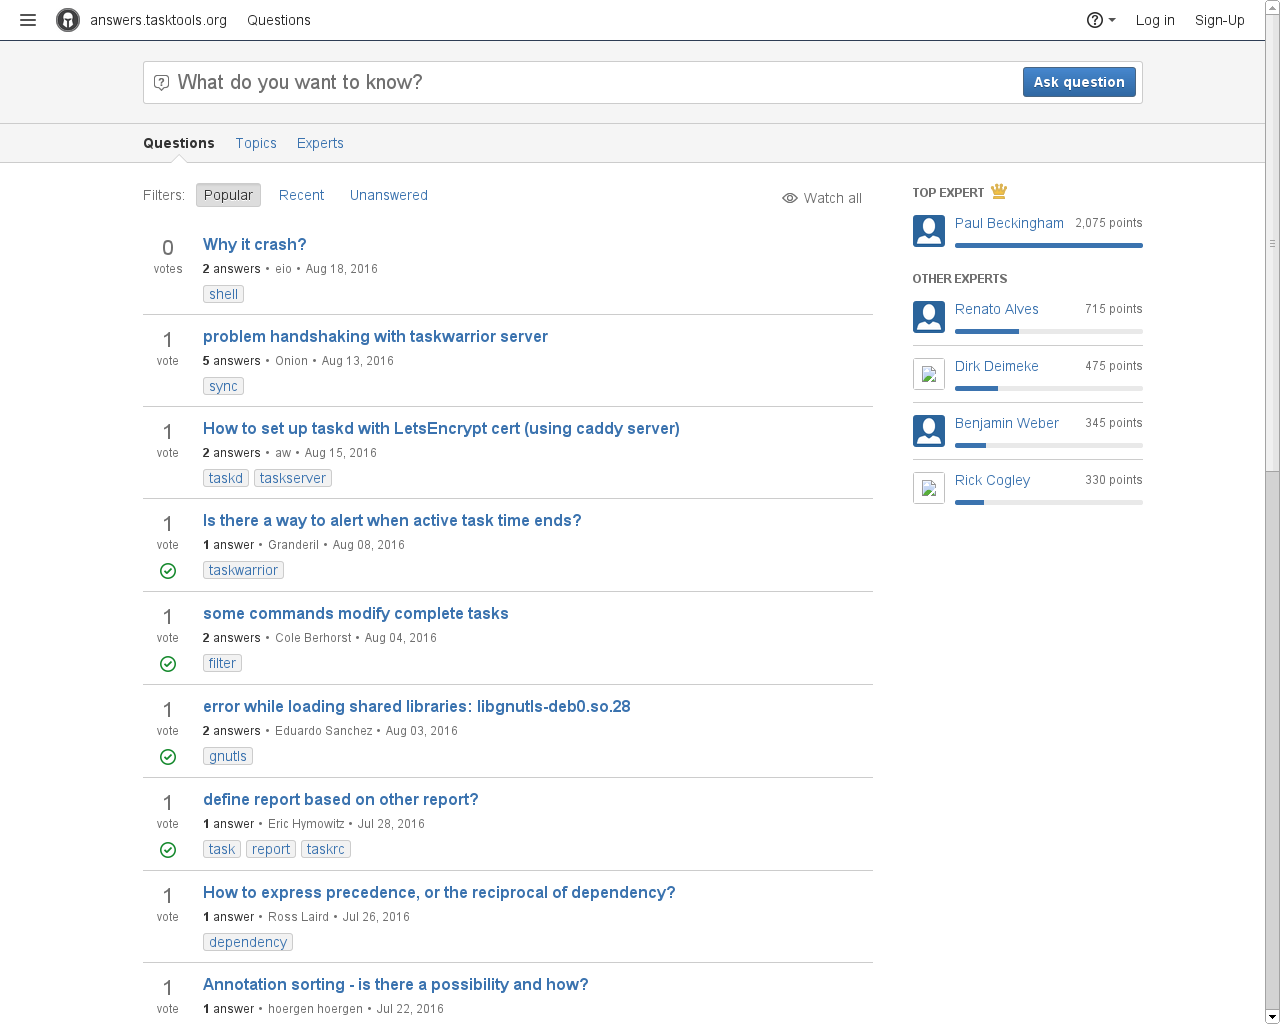
\includegraphics[width=10cm,height=7.5cm]{answers-tasktools-org.png}}
    \end{center}
\end{frame}

\begin{frame}\frametitle{status.tasktools.org -- status of the universe}
    \begin{center}
        \href{http://status.tasktools.org/}{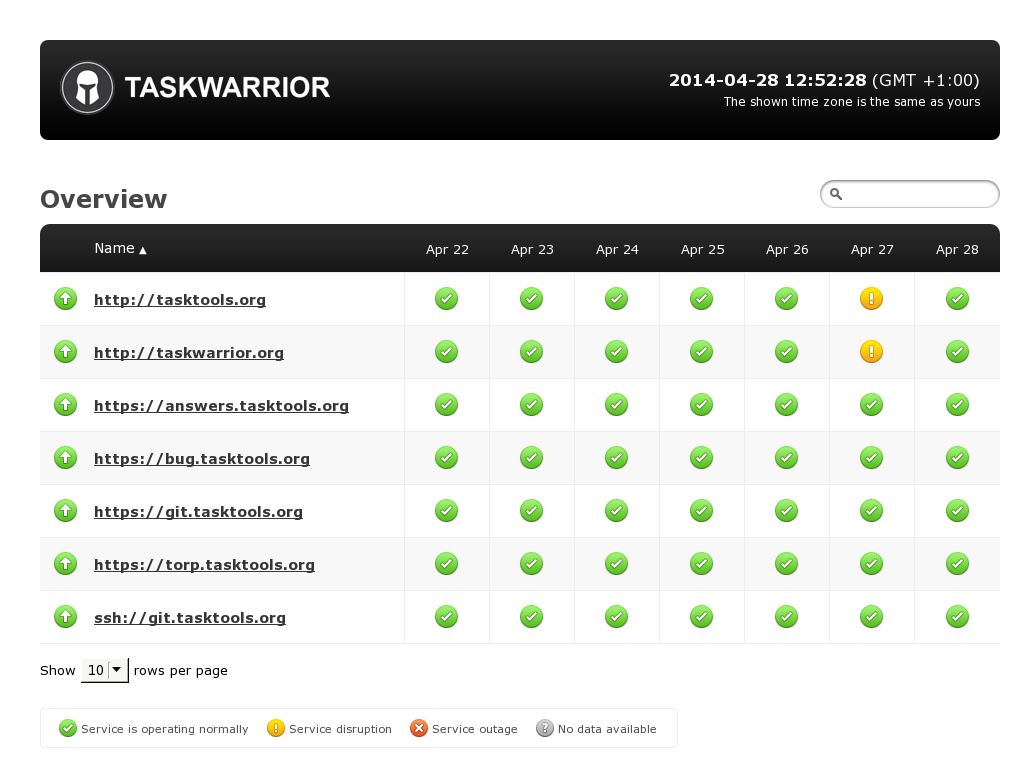
\includegraphics[width=10cm,height=7.5cm]{status-tasktools-org.png}}
    \end{center}
\end{frame}

\begin{frame}\frametitle{statuspage.tasktools.org -- more status}
    \begin{center}
        \href{http://statuspage.tasktools.org/}{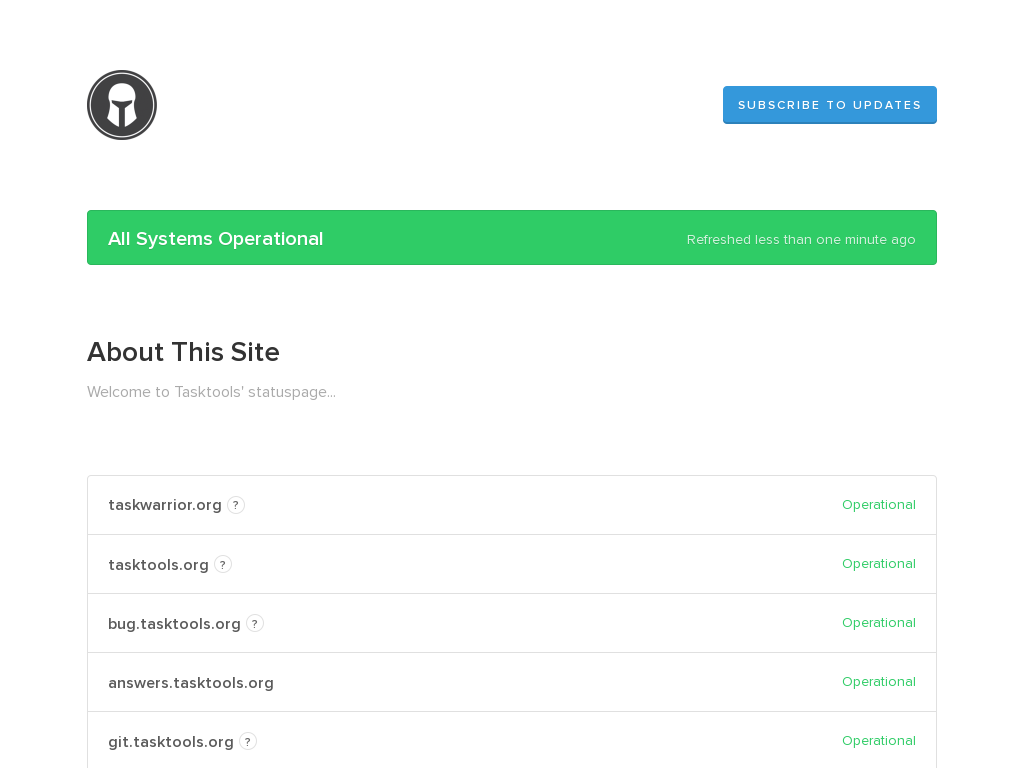
\includegraphics[width=10cm,height=7.5cm]{statuspage-tasktools-org.png}}
    \end{center}
\end{frame}

\begin{frame}\frametitle{bug.tasktools.org -- issue tracking}
    \begin{center}
        \href{https://bug.tasktools.org/}{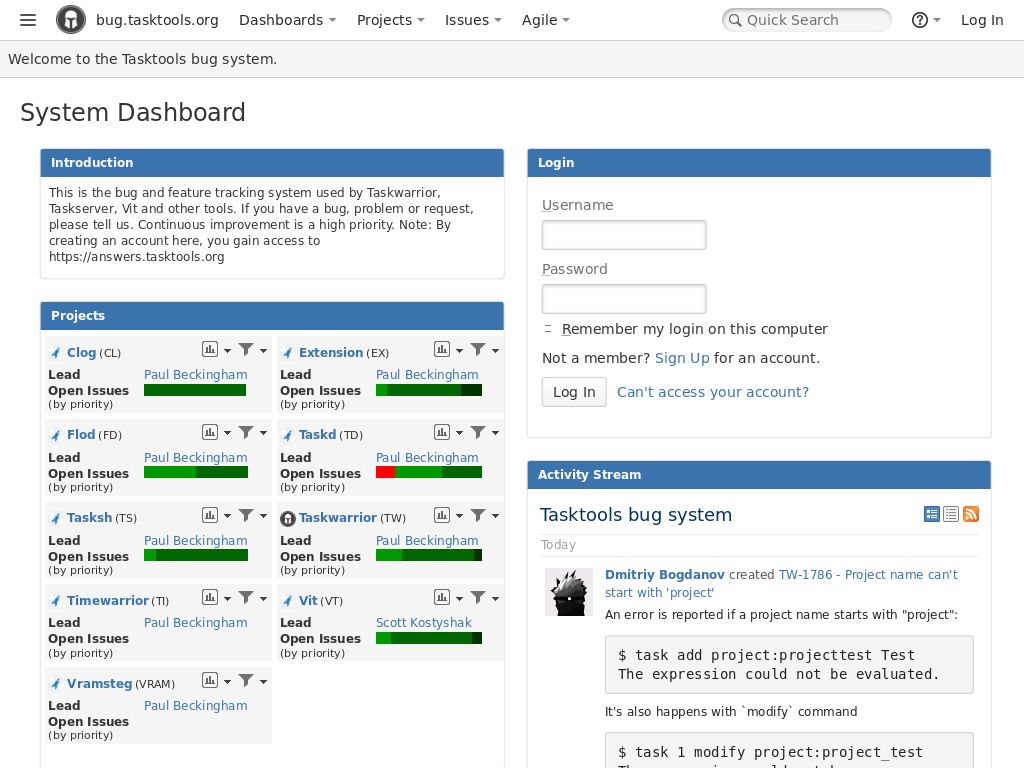
\includegraphics[width=10cm,height=7.5cm]{bug-tasktools-org.png}}
    \end{center}
\end{frame}

\begin{frame}\frametitle{git.tasktools.org -- repository management}
    \begin{center}
        \href{https://git.tasktools.org/}{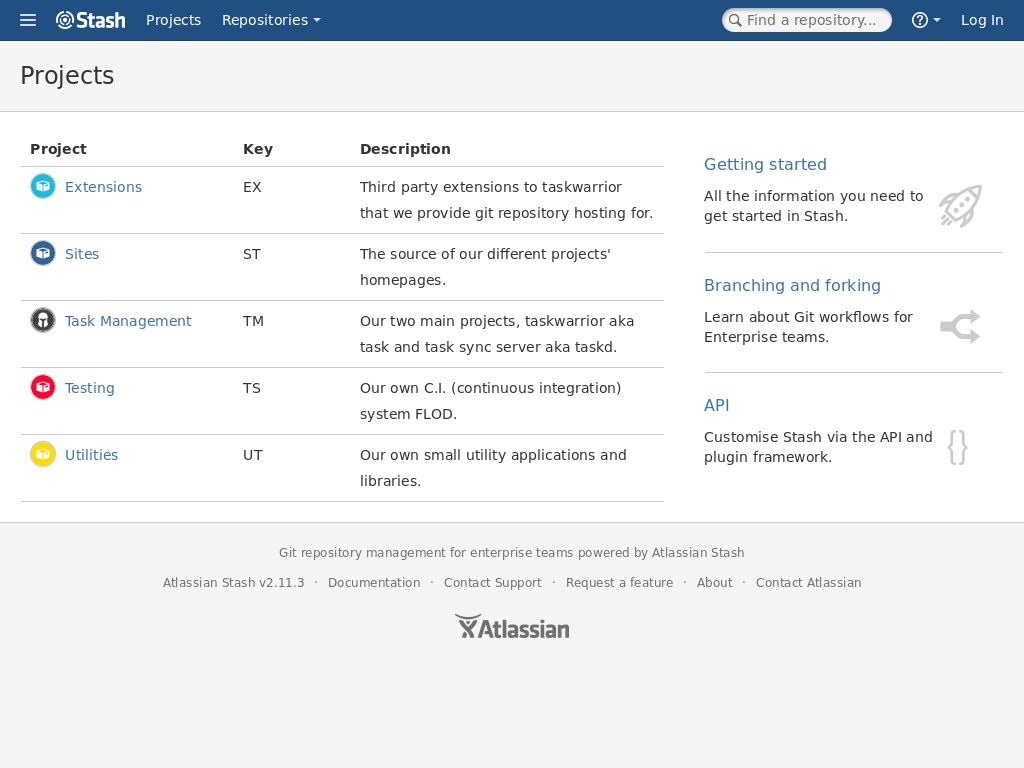
\includegraphics[width=10cm,height=7.5cm]{git-tasktools-org.png}}
    \end{center}
\end{frame}

\begin{frame}\frametitle{3rd Party Apps}
    \begin{center}
        \href{http://taskwarrior.org/tools/}{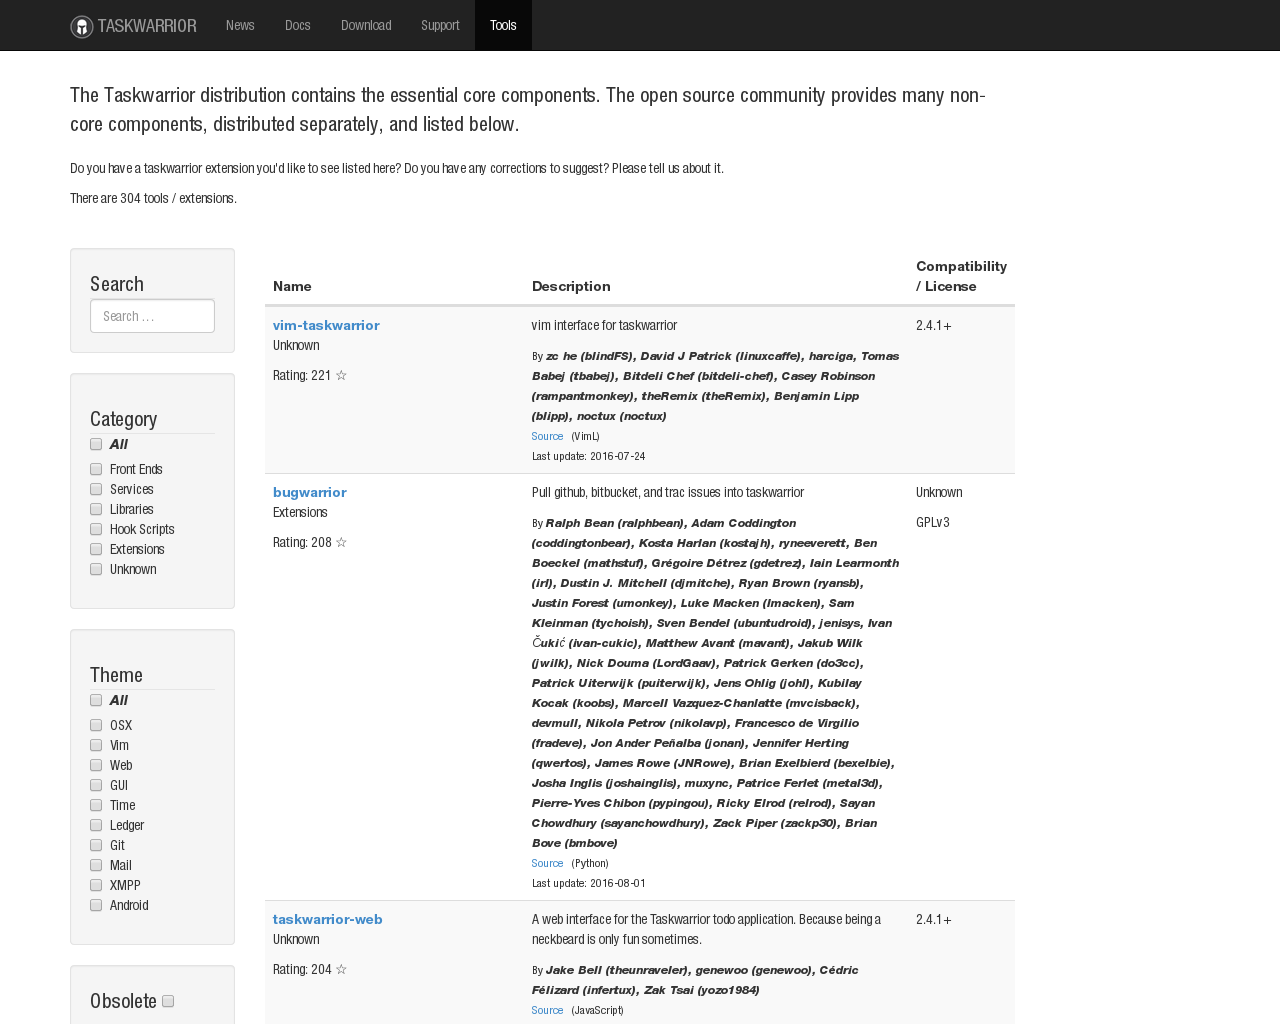
\includegraphics[width=10cm,height=7.5cm]{3rdparty.png}}
    \end{center}
\end{frame}

\begin{frame}\frametitle{tasktools.org -- collection of software}
    \begin{center}
        \href{http://tasktools.org/}{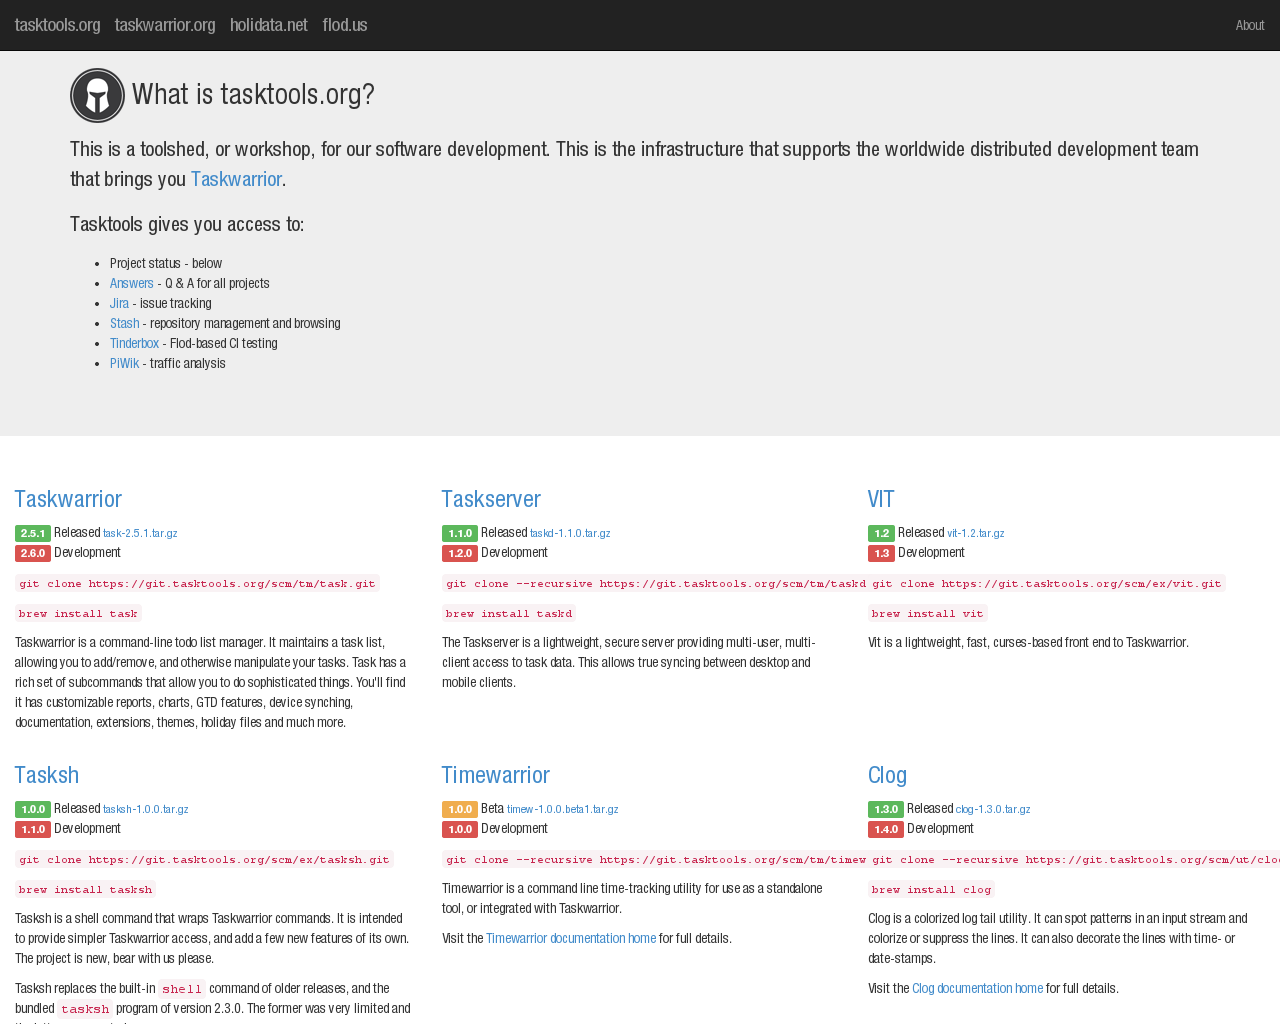
\includegraphics[width=10cm,height=7.5cm]{tasktools-org.png}}
    \end{center}
\end{frame}

\begin{frame}\frametitle{Timewarrior -- Time tracking}
    \begin{center}
        \href{http://taskwarrior.org/docs/timewarrior/index.html}{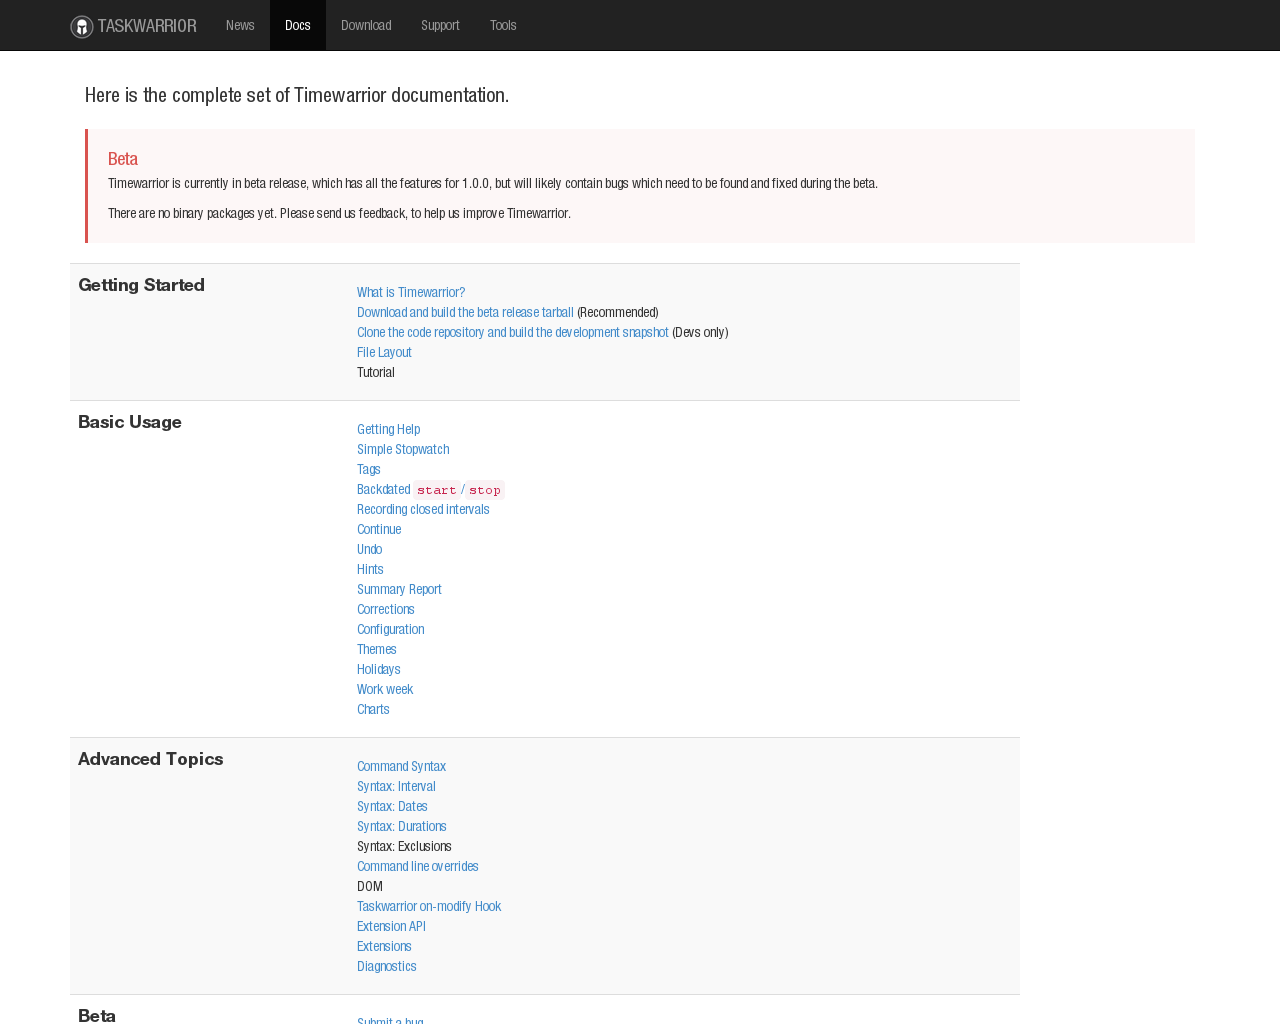
\includegraphics[width=10cm,height=7.5cm]{timewarrior.png}}
    \end{center}
\end{frame}

\begin{frame}\frametitle{VIT -- curses-based front end to Taskwarrior}
    \begin{center}
        \href{http://tasktools.org/projects/vit.html}{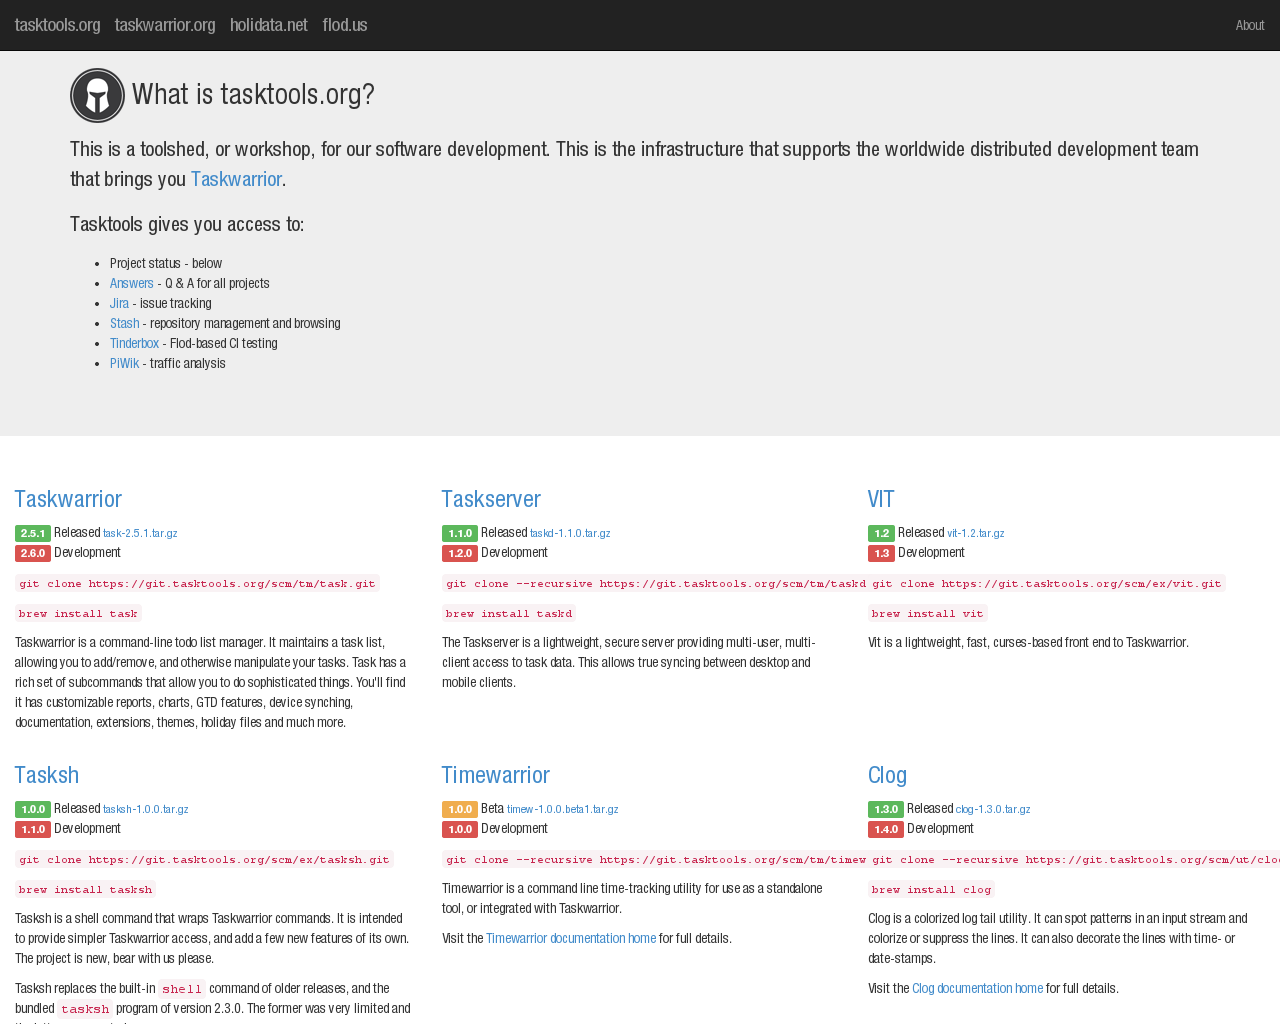
\includegraphics[width=10cm,height=7.5cm]{tasktools-org.png}}
    \end{center}
\end{frame}

\begin{frame}\frametitle{Tasksh -- Taskwarrior command wrapper}
    \begin{center}
        \href{http://tasktools.org/projects/tasksh.html}{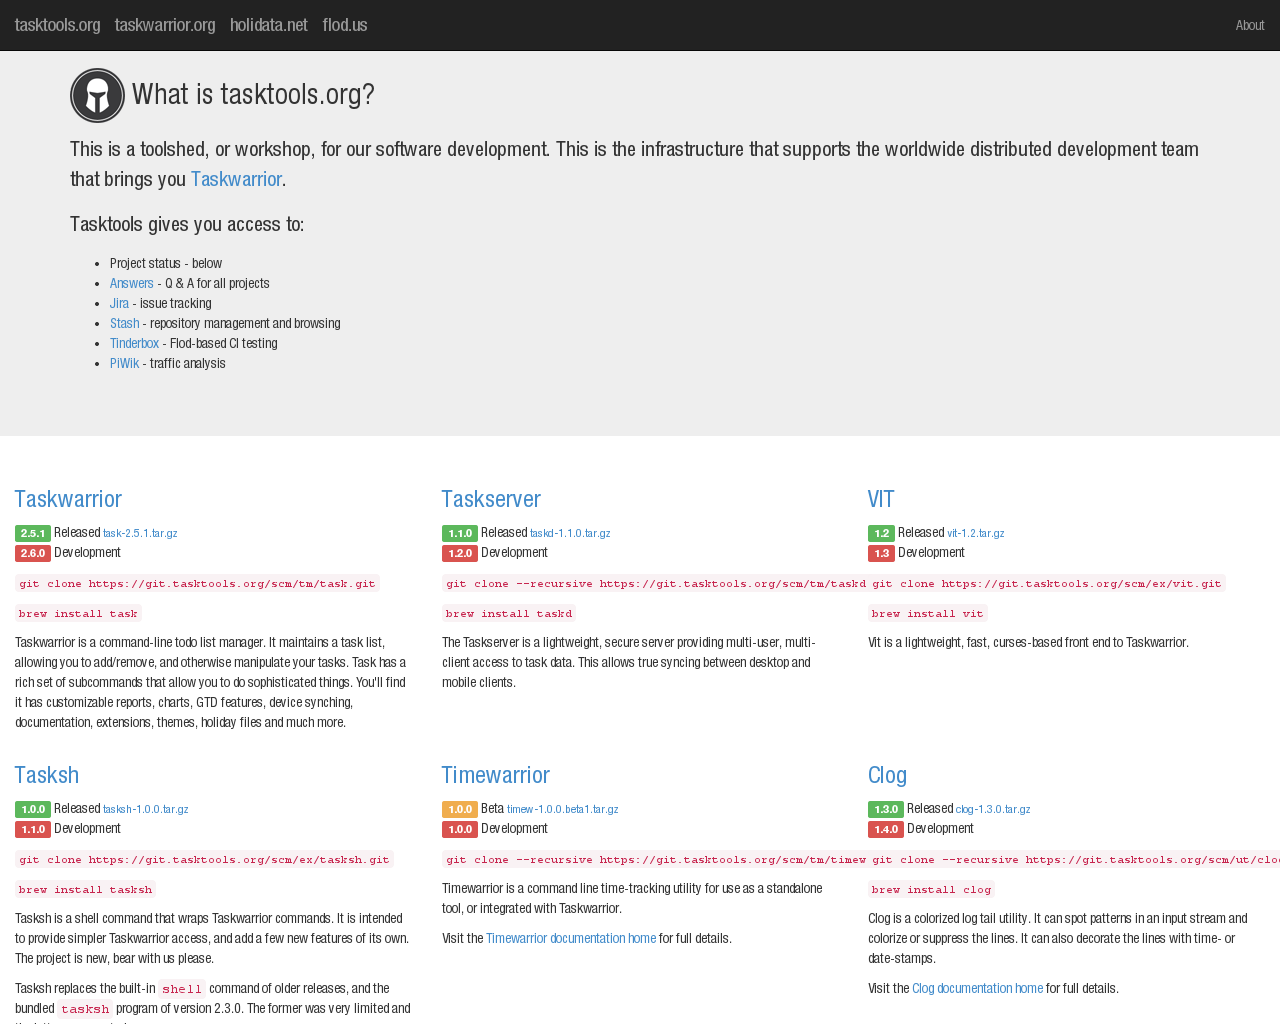
\includegraphics[width=10cm,height=7.5cm]{tasktools-org.png}}
    \end{center}
\end{frame}

\begin{frame}\frametitle{Clog -- colorized log tail utility}
    \vfill
    \begin{center}
        \href{http://tasktools.org/projects/clog.html}{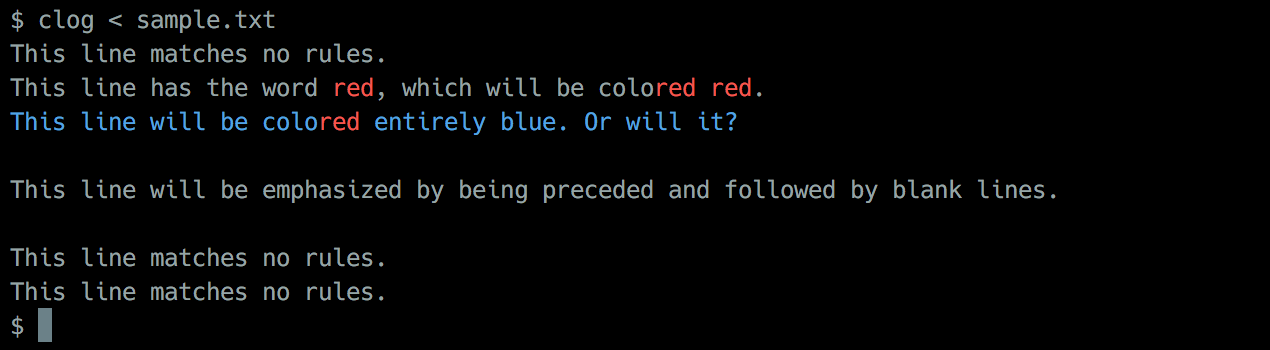
\includegraphics[width=10cm]{clog.png}}
    \end{center}
    \vfill
\end{frame}

\begin{frame}\frametitle{Vramsteg -- CLI progress bar}
    \begin{center}
        \href{http://tasktools.org/projects/vramsteg.html}{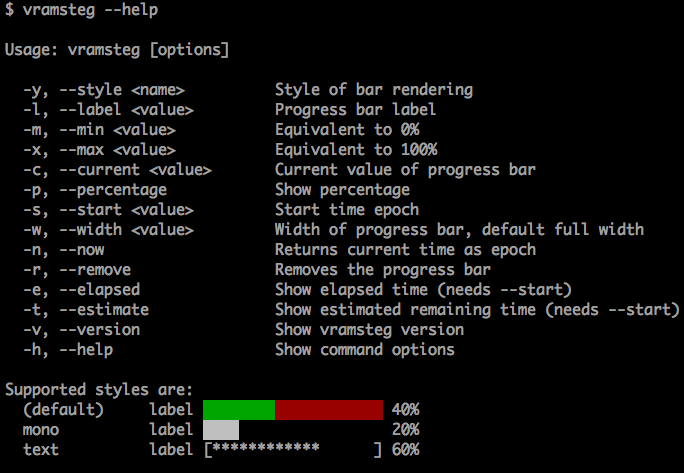
\includegraphics[width=10cm,height=7.5cm]{vramsteg.png}}
    \end{center}
\end{frame}

\begin{frame}\frametitle{Anomaly -- Data anomaly detection utility}
    \begin{center}
        \href{http://tasktools.org/projects/anomaly.html}{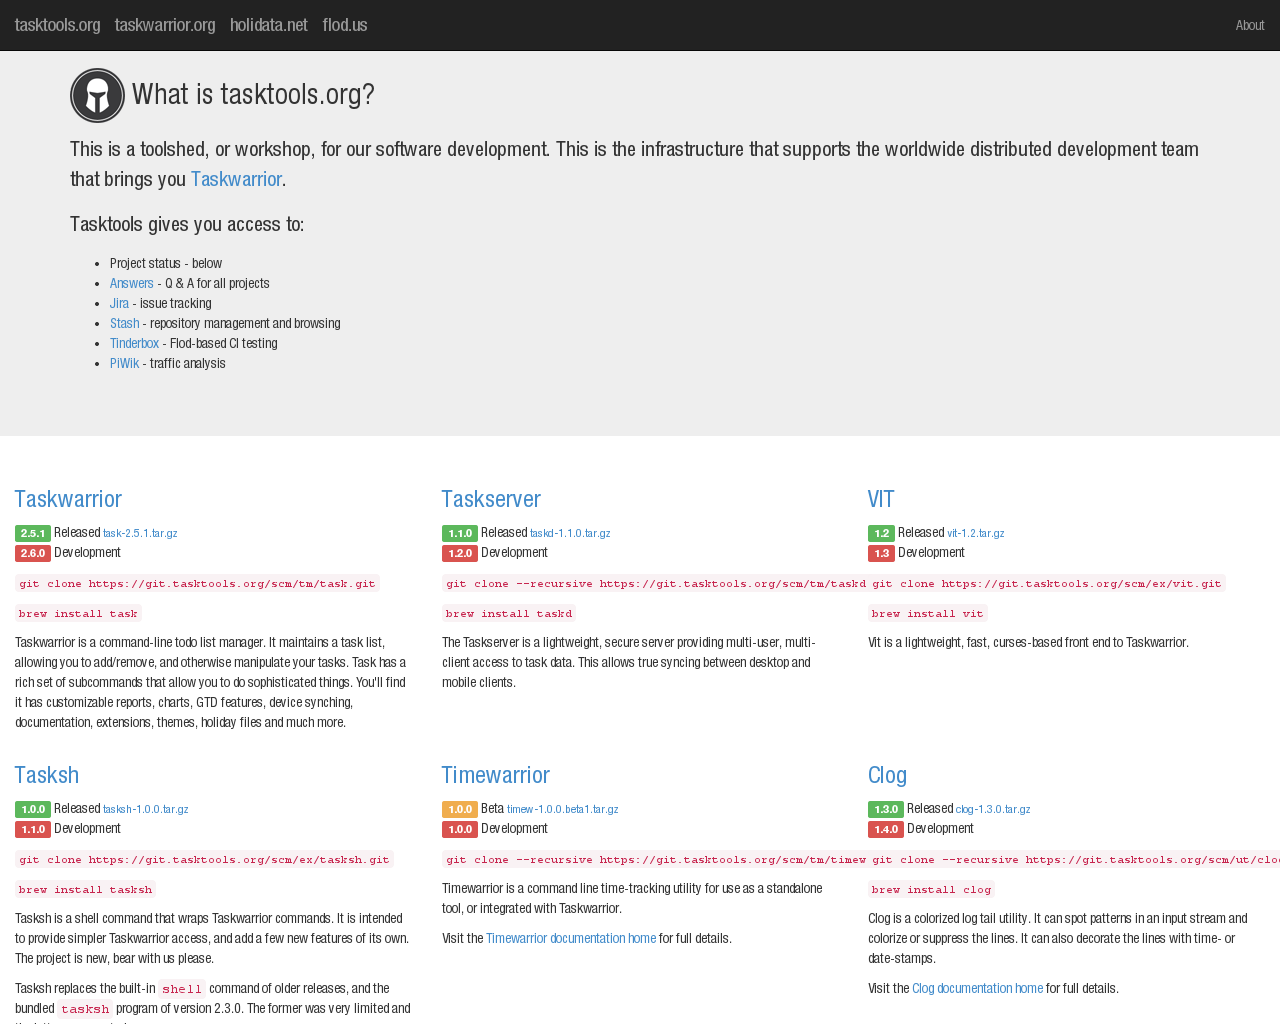
\includegraphics[width=10cm,height=7.5cm]{tasktools-org.png}}
    \end{center}
\end{frame}

\begin{frame}\frametitle{central.tasktools.org -- continous integration}
    \begin{center}
        \href{http://central.tasktools.org/}{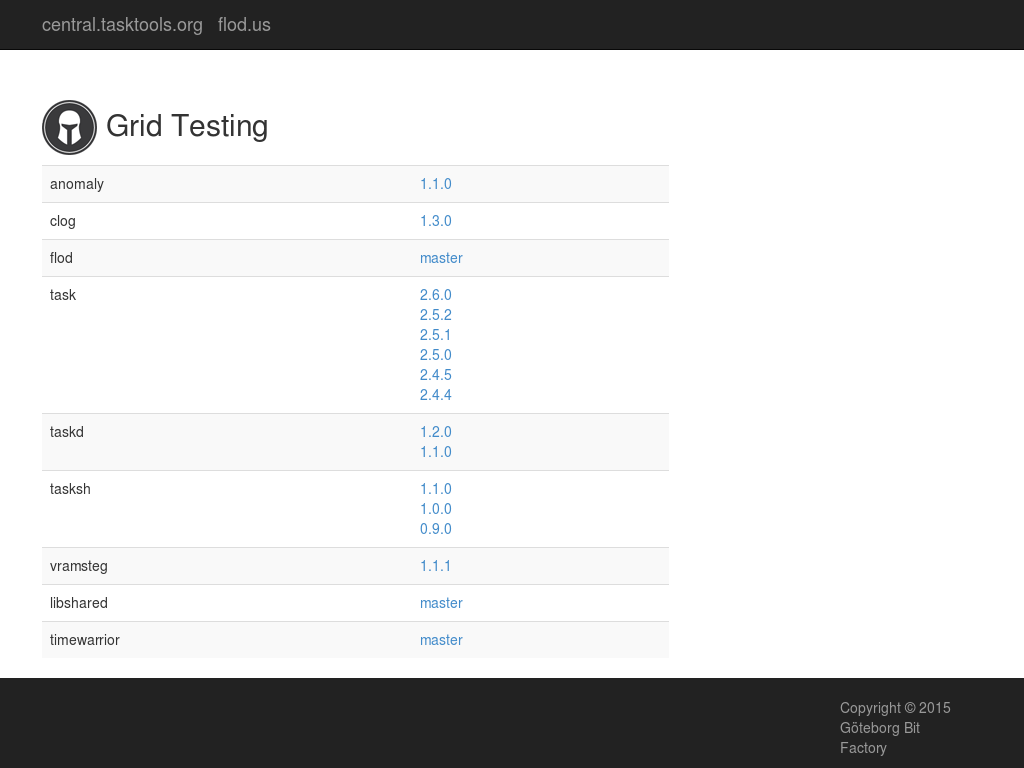
\includegraphics[width=10cm,height=7.5cm]{central-tasktools-org.png}}
    \end{center}
\end{frame}

\begin{frame}\frametitle{holidata.net -- holiday data for several countries}
    \begin{center}
        \href{http://holidata.net/}{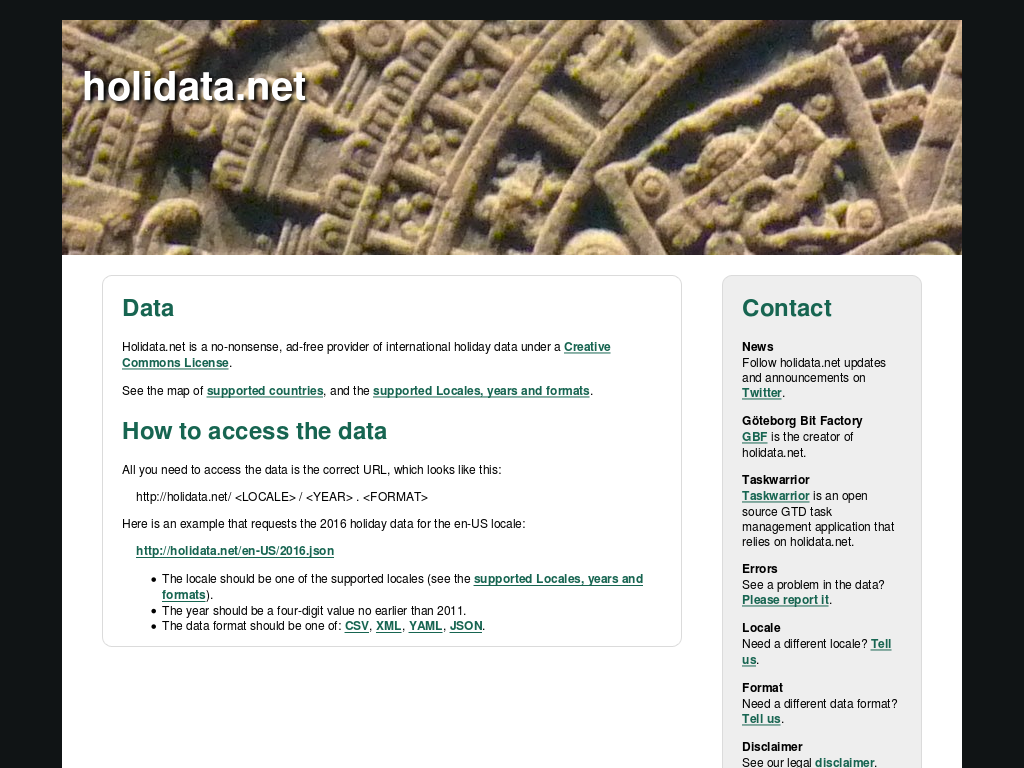
\includegraphics[width=10cm,height=7.5cm]{holidata-net.png}}
    \end{center}
\end{frame}

\begin{frame}\frametitle{flod.us -- continous integration framework}
    \begin{center}
        \href{http://flod.us/}{
\includegraphics[width=10cm,height=7.5cm]{flod-us.png}}
    \end{center}
\end{frame}

\begin{frame}\frametitle{torp.tasktools.org}
    \begin{center}
        \href{https://torp.tasktools.org}{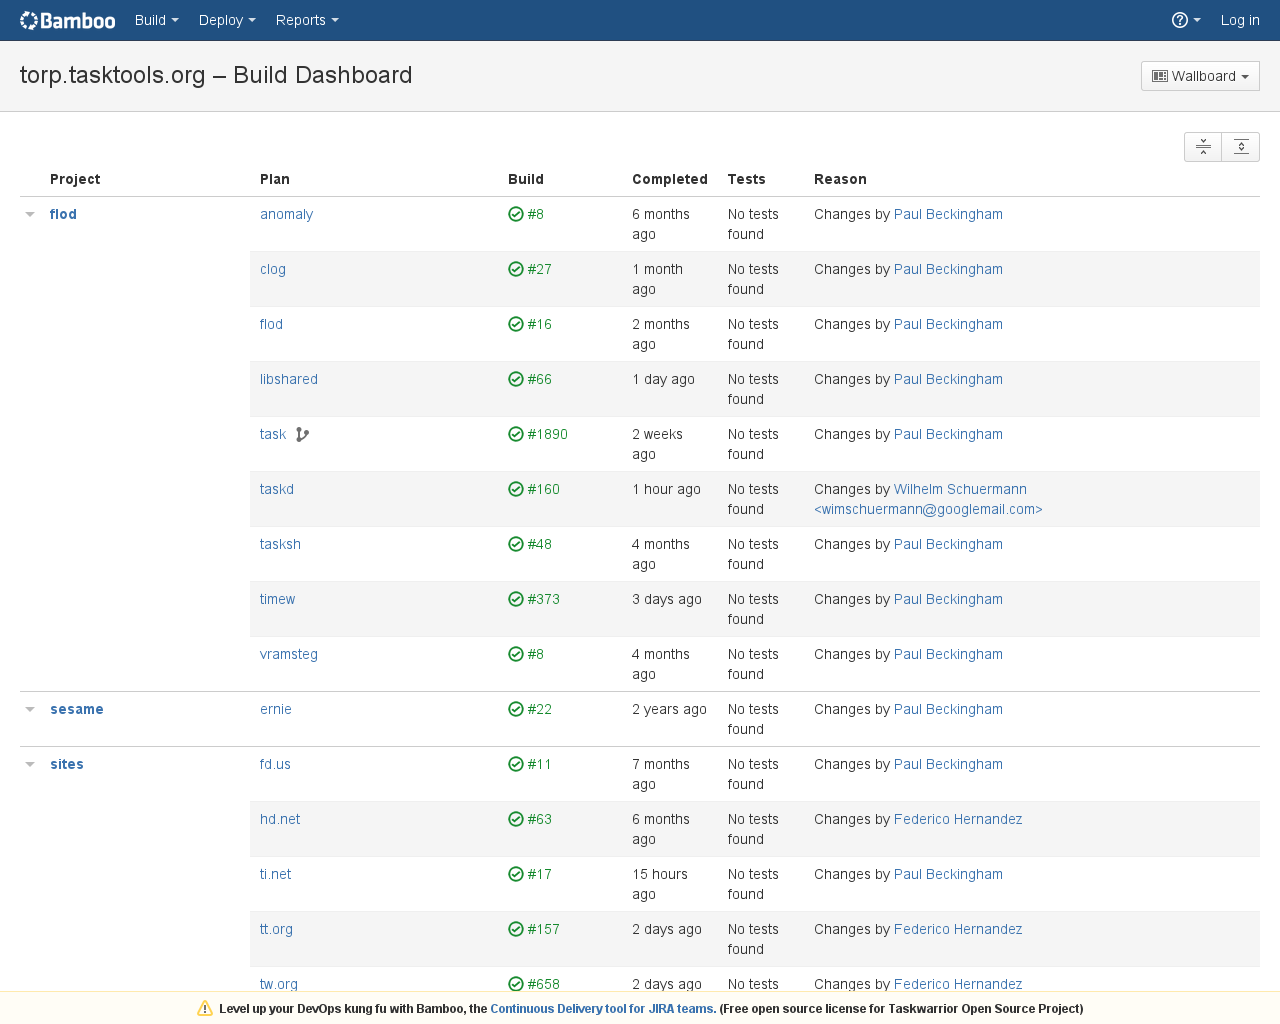
\includegraphics[width=10cm,height=7.5cm]{torp-tasktools-org.png}}
    \end{center}
\end{frame}

\begin{frame}\frametitle{botbot.me -- IRC channel logger}
    \begin{center}
        \href{https://botbot.me/freenode/taskwarrior/}{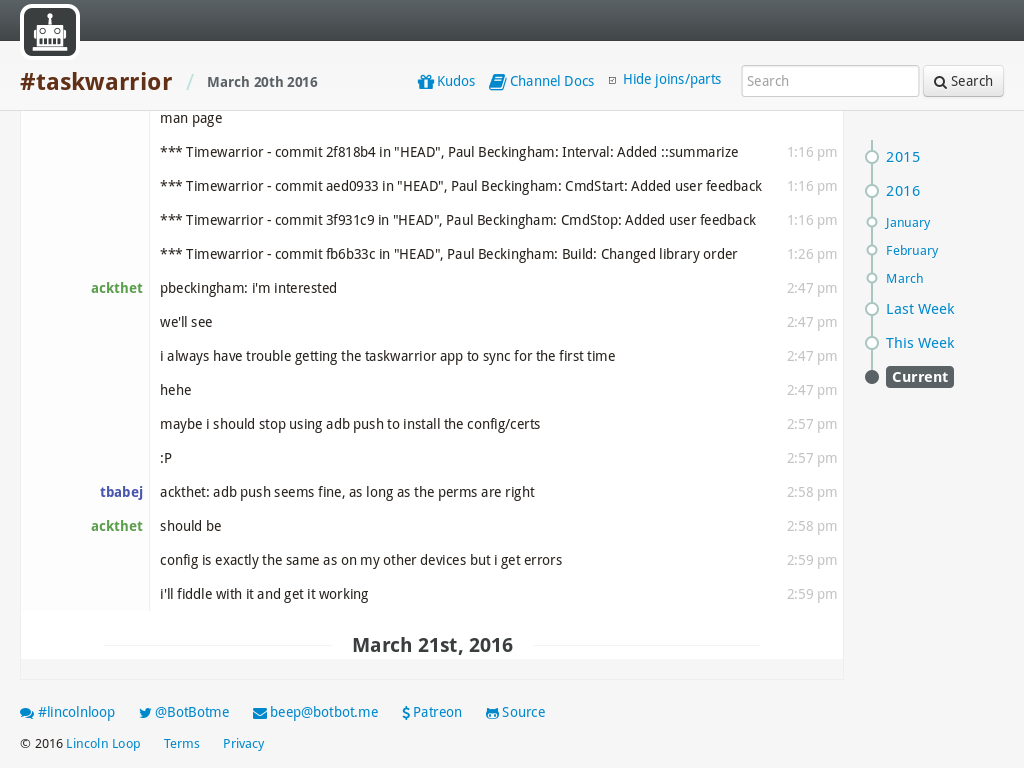
\includegraphics[width=10cm,height=7.5cm]{botbot-me-taskwarrior.png}}
    \end{center}
\end{frame}

% \begin{frame}\frametitle{Twitter -- no spam (promised!)}
%     \begin{center}
%         \href{https://twitter.com/taskwarrior}{
\includegraphics[width=10cm,height=7.5cm]{twitter-taskwarrior.png}}
%     \end{center}
% \end{frame}

\begin{frame}[fragile]\frametitle{Thanks for your patience!}
    \vfill
    \begin{center}
        Dirk Deimeke, Taskwarrior-Team, 2016, \href{https://creativecommons.org/licenses/by/4.0/}{CC-BY}

        \href{mailto:dirk@deimeke.net}{dirk@deimeke.net}

        \href{https://d5e.org/}{d5e.org}
    \end{center}
\end{frame}

\end{document}
